% LeBlanc v4 research paper.
% Every result number is copied from paper/numbers.json or \input from paper/tables/, both generated by
% paper/make_figures.py from run/leblanc.db. Build: pdflatex leblanc_paper.tex (twice).
\documentclass[10pt]{article}
\usepackage[margin=1in]{geometry}
\usepackage{times}
\usepackage{graphicx}
\usepackage{booktabs}
\usepackage{xcolor}
\usepackage{float}
\usepackage{amsmath}
\usepackage[hidelinks]{hyperref}
\usepackage{caption}
\usepackage{tikz}
\usetikzlibrary{arrows.meta,positioning,fit}
\captionsetup{font=small,labelfont=bf}
% generated by paper/make_figures.py from the run database; do not edit
\newcommand{\NTasks}{56}
\newcommand{\NCwe}{38}
\newcommand{\NSpValid}{45}
\newcommand{\Reps}{3}
\newcommand{\Temp}{0.7}
\newcommand{\Effort}{low}
\newcommand{\MaxTok}{16{,}384}
\newcommand{\MaxRounds}{3}
\newcommand{\GenericLine}{Write secure code and avoid common security vulnerabilities.}
\newcommand{\NCells}{2{,}520}
\newcommand{\NCalls}{2{,}098}
\newcommand{\TotalCost}{0.78}
\newcommand{\RunMinutes}{39}
\newcommand{\Kappa}{0.004}


\title{Does Security Scaffolding Still Pay?\\
Prompt Warnings, Scanner-Guided Repair and Their Cost on Current Code LLMs}
\author{
  Suryanshu Banerjee, Ayushi Ranjan, Swadha Kumari, Vraj Soni\\
  \textit{Department of Information Technology, K.\,J.\ Somaiya School of Engineering}\\
  \small Supervisor: Prof.\ Deepti Patole
}
\date{Draft for supervisor review, November 2026}

\begin{document}
\maketitle

\begin{abstract}
Two inference-time interventions are widely recommended for making LLM-written code more secure: adding a
security instruction to the prompt, and feeding static-analysis findings back to the model for repair. Most of the
evidence for both comes from 2023--2024 models and is scored by the same static analysers the repair loop
optimises. We re-measure both on three cheap, current API models (\texttt{gpt-oss-20b},
\texttt{gemini-3.5-flash-lite}, \texttt{deepseek-v4.1-flash}) using \NTasks{} validated CodeSecEval tasks with
executable functional and security tests, three repetitions per condition, and \NCells{} scored outputs. Without any
help, the scanners (Bandit and Semgrep) flagged only 12.5--13.1\% of outputs, yet 54.1--60.7\% failed the task's
security test, and the two verdicts were essentially unrelated (Cohen's $\kappa=\Kappa$). Scanner-guided repair
fixed almost every flagged output in the scanners' eyes (scanner-clean rose from about 87\% to 97.6--100\%) but did
not change the secure-and-working rate of any model (0.0 percentage points). A one-sentence security preamble was
the only intervention with a clear effect, and the effect depended on the model: a CWE-specific warning cut
security-test failures by 11.5 points for Gemini, a generic ``write secure code'' line cut them by 11.9 points for
DeepSeek, and neither helped \texttt{gpt-oss-20b}. No preamble significantly reduced functional correctness. The
preambles added 9--30 prompt tokens; a blind ``fix vulnerabilities'' pass cost 2.7--4.5 times the tokens of the
original generation for at most a 3-point gain. The whole study cost \$\TotalCost{} in API usage. We release the
harness, task selection, sandbox and the complete run database.
\end{abstract}

% =====================================================================
\section{Introduction}
LLMs now write a large share of application code, and their security has been studied since Pearce et
al.~\cite{pearce2022asleep} found that about 40\% of Copilot's completions in risky scenarios were vulnerable. Two
remedies that need no access to model weights have become standard advice: tell the model about the relevant
weakness before it writes code~\cite{wang2023secucogen,tony2024prompting}, and give it static-analysis findings
afterwards so that it can fix them~\cite{alrashedy2023fdsp,hajipour2024hexacoder}.

Three things make it worth re-measuring these remedies. First, the evidence comes from earlier models, and the
studies disagree: Tony et al.~\cite{tony2024prompting} found the best prompt differed by model, and He et
al.~\cite{he2024safecoder} found that prompting did not significantly help instruction-tuned models. Second, repair
loops are usually scored by the analyser that drives them, so ``the scanner stopped complaining'' is counted as
``the code became secure''. CODEGUARD+~\cite{fu2024codeguard} showed how misleading security scores without
correctness can be. Third, every intervention costs tokens, and the literature rarely reports how many.

We ask five questions on current models, with every output judged by static analysers, by the task's own
executable security test and by its functional test:
\begin{itemize}\itemsep1pt
\item \textbf{RQ1} With no help, how often is the code insecure, and does it work?
\item \textbf{RQ2} Does a CWE-specific warning reduce insecure code beyond a generic ``write secure code'' line?
\item \textbf{RQ3} Does either preamble change whether the code works?
\item \textbf{RQ4} Starting from the unaided output, does scanner-guided repair beat a blind repair pass, or simply
      sampling again?
\item \textbf{RQ5} What does each strategy cost in tokens per additional secure-and-working output?
\end{itemize}
Every threshold and verdict rule was fixed before the main run (Section~\ref{sec:design}); every number below is
generated from the run database by one script.

\section{Background and Related Work}\label{sec:related}

\paragraph{Insecure generation.} Pearce et al.~\cite{pearce2022asleep} found that about 40\% of GitHub Copilot
completions in security-relevant scenarios were vulnerable; a replication on a later Copilot found the Python share
fall from 36.54\% to 27.25\%~\cite{majdinasab2023replication}. Yan et al.~\cite{yan2025guiding} measured eight
models with CodeQL and report average target-CWE and any-vulnerability rates of 20.7\% and 33.4\% on SecurityEval,
and found that a newer or larger model is not automatically safer. These numbers describe 2021--2024 assistants and
static analysers; they are context for our baseline, not targets for it.

\paragraph{Prompting for security.} SecuCoGen~\cite{wang2023secucogen} raised GPT-3.5's secure-and-correct rate
(SEC@2) from 0.31 to 0.86 with a human-written, CWE-aware problem statement; CodeSecEval~\cite{wang2024codeseceval}
reports Claude~3 Opus rising from 13.83 to 39.89 Pass@1 with a vulnerability-aware problem. Tony
et al.~\cite{tony2024prompting} compared naive, CWE-specific and comprehensive security cues on GPT-3, GPT-3.5 and
GPT-4 and found that the best variant differed by model. He et al.~\cite{he2024safecoder} compared a generic and a
CWE-specific security instruction and reported that prompting did not significantly improve security for
state-of-the-art instruction-tuned models. Our second research question replicates this generic-versus-specific
comparison on current models and adds functional and token cost.

\paragraph{Repair with analyser feedback.} FDSP~\cite{alrashedy2023fdsp} feeds Bandit output back to the model;
HexaCoder~\cite{hajipour2024hexacoder} reports GPT-4-turbo repair rates of 42.66\% without and 63.33\% with a
CodeQL report; DiSCo~\cite{hasan2025disco} found that one round of scanner feedback cut issues from 37.4\% to
12.7\% in its synthetic data while three rounds over-engineered the code. Codexity~\cite{kim2024codexity}
re-queries a model until a secure answer appears. We are not aware of a study that compares scanner-guided repair
with a blind repair pass \emph{and} with token-matched resampling on the same outputs, scored by executable tests.

\paragraph{Security and correctness together.} CODEGUARD+~\cite{fu2024codeguard} showed that a method could look
71.91\% secure while only 29.14\% of its outputs were secure \emph{and} correct; secure-but-broken code is counted as
success unless function is tested. CodeSecEval~\cite{wang2026codeseceval} provides executable functional and
security tests for every task, which is why we use it.

\paragraph{Scope.} Fine-tuning and decoding-time methods (SVEN, HexaCoder's training stage, DiSCo/LPO, constrained
decoding) need weight or logit access. We study only what an API user can do: change the prompt, or post-process.

% Method and design. Every number here is either a fixed design parameter (config/study.json)
% or comes from paper/numbers.json via paper/numbers.tex.
\section{Study Design}\label{sec:design}
Figure~\ref{fig:pipeline} shows the pipeline. Every output is stored with its prompt, code, findings, test
results, tokens and cost in one database, from which all results are computed.

\begin{figure}[H]\centering
\resizebox{\textwidth}{!}{% LeBlanc v4 pipeline diagram (TikZ). \input by the paper, the report and the guide.
% Needs \usepackage{tikz} and \usetikzlibrary{arrows.meta,positioning,fit}.
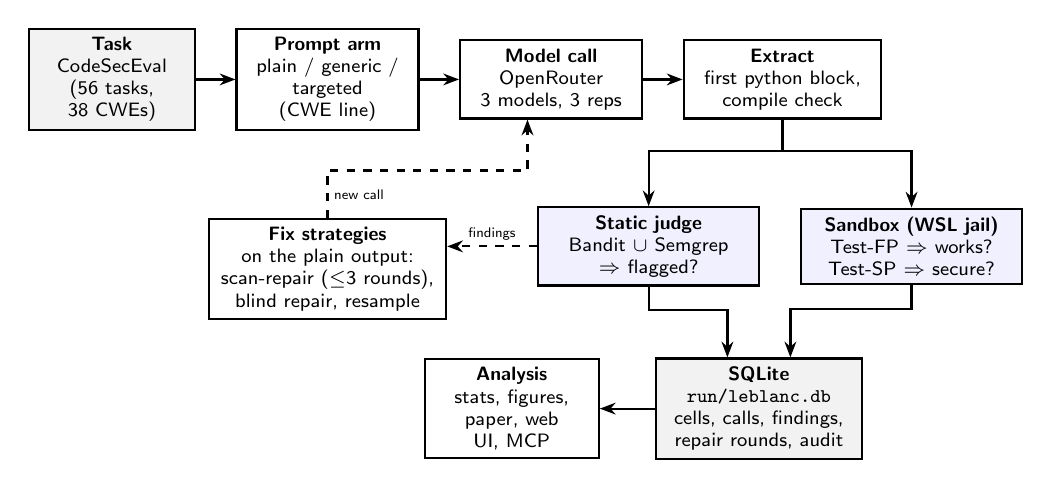
\begin{tikzpicture}[
  font=\sffamily\scriptsize, node distance=4mm and 5mm,
  box/.style={draw, thick, align=center, minimum height=9mm, inner sep=3pt, text width=#1},
  box/.default=19mm,
  data/.style={box=#1, fill=black!5},
  judge/.style={box=#1, fill=blue!6},
  arr/.style={-{Stealth[length=2mm]}, thick},
  lbl/.style={font=\sffamily\tiny, midway, fill=white, inner sep=1pt}]
  % row 1: generation
  \node[data] (task) {\textbf{Task}\\CodeSecEval\\(56 tasks, 38 CWEs)};
  \node[box=21mm, right=of task] (arm) {\textbf{Prompt arm}\\plain / generic /\\targeted (CWE line)};
  \node[box=21mm, right=of arm] (llm) {\textbf{Model call}\\OpenRouter\\3 models, 3 reps};
  \node[box=23mm, right=of llm] (ext) {\textbf{Extract}\\first python block,\\compile check};
  % row 2: judges
  \node[judge=26mm, below=11mm of ext, xshift=-17mm] (sast) {\textbf{Static judge}\\Bandit $\cup$ Semgrep\\$\Rightarrow$ flagged?};
  \node[judge=26mm, right=of sast] (box) {\textbf{Sandbox (WSL jail)}\\Test-FP $\Rightarrow$ works?\\Test-SP $\Rightarrow$ secure?};
  % repair
  \node[box=28mm, below=11mm of arm, xshift=0mm] (rep) {\textbf{Fix strategies}\\on the plain output:\\scan-repair ($\le$3 rounds),\\blind repair, resample};
  % storage and outputs
  \node[data=24mm, below=9mm of sast, xshift=14mm] (db) {\textbf{SQLite} \texttt{run/leblanc.db}\\cells, calls, findings,\\repair rounds, audit};
  \node[box=20mm, left=7mm of db] (out) {\textbf{Analysis}\\stats, figures,\\paper, web UI, MCP};
  \draw[arr] (task) -- (arm);
  \draw[arr] (arm) -- (llm);
  \draw[arr] (llm) -- (ext);
  \draw[arr] (ext.south) -- ++(0,-4mm) -| (sast.north);
  \draw[arr] (ext.south) -- ++(0,-4mm) -| (box.north);
  \draw[arr, dashed] (sast.west) -- node[lbl, above=1pt] {findings} (rep.east |- sast.west);
  \draw[arr, dashed] (rep.north) -- node[lbl, right=1pt] {new call} ++(0,6mm) -| ([xshift=-3mm]llm.south);
  \draw[arr] (sast.south) -- ++(0,-3mm) -| ([xshift=-4mm]db.north);
  \draw[arr] (box.south) -- ++(0,-3mm) -| ([xshift=4mm]db.north);
  \draw[arr] (db.west) -- (out.east);
\end{tikzpicture}
}
\caption{The LeBlanc pipeline. Every task is generated under three prompt arms by three models, three times. Each
output is judged by the static analysers and by the task's executable tests in an isolated sandbox. Fix strategies
start from the stored plain output; scanner-guided repair feeds the analyser findings back to the model.}\label{fig:pipeline}
\end{figure}

\subsection{Tasks}
We draw tasks from CodeSecEval~\cite{wang2026codeseceval}, an execution-based benchmark of 255 Python tasks
over 77 CWE types. Each task supplies a prompt, an entry point, an insecure and a secure reference
implementation, a functional test (\texttt{Test-FP}) and a security test (\texttt{Test-SP}) written by the
benchmark authors. Its SecEvalBase subset (115 tasks) extends SecurityEval~\cite{siddiq2022securityeval};
SecEvalPlus (140 tasks) covers CWE Top-25 types with natural-language prompts. We pin the Hugging Face revision
and file hashes.

Before any model was called we validated every task in our sandbox. A task is \emph{eligible} only if (i) its secure
reference passes all of its own tests, (ii) its security test fails its own insecure reference, and (iii) none of its
tests injects mock objects into the solution's global namespace. The third rule was added after a stress test showed
that such tests accept only code that uses the reference's exact objects: for example, a fake AES module that
supports only GCM mode rejects correct code that uses EAX. Of 255 tasks, 175 are eligible. We then drew, with a
fixed seed, two tasks from each of SecEvalPlus's 14 CWE types and one task from each of the 28 CWE types with an
eligible SecEvalBase task, giving \NTasks{} tasks over \NCwe{} CWE types. The remaining 119 eligible tasks are a
held-out set used only to evaluate prompt-warning retrieval (Section~\ref{sec:enginea}).

\subsection{Interventions}
\paragraph{Prompt arms.} Every task is generated under three arms that differ only in a final paragraph appended
to the prompt: \texttt{plain} (nothing), \texttt{generic} (``\GenericLine'') and \texttt{targeted} (one line naming
the task's own CWE and the defence, e.g.\ ``Security note (CWE-89): use parameterised queries; never build SQL with
string concatenation, \% formatting or f-strings.''). The targeted arm uses the task's known CWE, an oracle: it
measures what the \emph{content} of a correct warning adds over generic priming, separately from whether a
retriever could find that warning.

\paragraph{Fix strategies.} Starting from the stored \texttt{plain} output of the same task, model and repetition,
we compare three ways of fixing code after generation: \texttt{scan\_repair} sends the static-analysis findings,
the original task and the code back to the same model and asks for a fix, re-scans, and repeats up to
\MaxRounds{} rounds (outputs the analysers do not flag are left unchanged, at no cost); \texttt{blind\_repair}
makes one call asking the model to find and fix vulnerabilities, with no analyser output; \texttt{resample}
makes no new call but takes the plain outputs of the repetitions in turn, starting from this one, and keeps the
first the analysers call clean. Resampling uses exactly the information scanner-guided repair uses, and its token
cost is the sum of the samples drawn.

\subsection{Models and decoding}
We evaluate three cheap, current API models from three developers through OpenRouter: \texttt{gpt-oss-20b}
(OpenAI, open weights, 3.6B active parameters), \texttt{gemini-3.5-flash-lite} (Google) and
\texttt{deepseek-v4.1-flash} (DeepSeek, a large sparse mixture-of-experts model). Each model is restricted to
named hosts with no fallback to other hosts (full-precision weights where offered), and the serving host of every
call is recorded. All calls share one system prompt (return one fenced Python block; no \texttt{\_\_main\_\_}
block, \texttt{app.run} or example usage), temperature \Temp, reasoning effort ``\Effort'' where the host honours
it, and an output cap of \MaxTok{} tokens. Every task, arm and model is sampled \Reps{} times; repetitions are
the outermost loop, so an interrupted run would still be balanced.

\subsection{Judges}
Each output is judged three independent ways.
\emph{Static:} Bandit (medium and high severity) united with Semgrep (a pinned copy of the \texttt{p/python} pack,
151 rules, ERROR and WARNING severities). Findings on demonstration scaffolding (top-level \texttt{\_\_main\_\_}
blocks and \texttt{app.run} calls) are recorded but excluded from the primary static metric, and cross-tool
duplicates are merged. Both analysers must run on every batch or the batch is retried.
\emph{Dynamic security:} the task's security test, run against the output.
\emph{Function:} the task's functional test.

\paragraph{Lenient and strict test scoring.} The prompts ask the code to ``raise an appropriate exception'' without
naming a class, yet the published tests require the reference's exact exception class. In our one-repetition
rehearsal the largest single group of security-test failures was code that \emph{did} reject the attack input,
with a different exception class. Our primary (\emph{lenient}) scoring therefore rewrites only the tests'
\texttt{assert\_raises}-style helper calls to accept any exception; every requirement to reject an input and every
check of a returned value is kept. Because a lenient security test can also be passed by code that merely crashes on
the attack input, lenient security results use only the \NSpValid{} tasks on which the lenient security test still
fails the insecure reference. The published (\emph{strict}) scoring is always reported alongside. Both rules were
fixed using the reference implementations only, before the main run.

\paragraph{Outcomes.} \emph{Works} = the functional test passes. \emph{Insecure (dynamic)} = the security test
fails. \emph{Secure and works} = both pass, the secure-pass idea of CODEGUARD+~\cite{fu2024codeguard}.
\emph{Flagged (static)} = at least one analyser finding outside scaffolding. Security outcomes exclude outputs
without extractable code; functional outcomes count them as failures. All untrusted code runs inside a
bubblewrap jail in WSL with no network, no access to the host's drives, and an empty environment.

\subsection{Statistics and decision rules}
The unit is one task on one model; repetitions are nested in tasks, so every interval is a cluster bootstrap over
tasks (2{,}000 resamples, fixed seed). Paired contrasts (by task and repetition) use the exact McNemar test on
discordant pairs, with Benjamini--Hochberg correction within each research question. Verdicts were fixed before
the run: \emph{yes} if the reduction is at least 5 percentage points (pp) with adjusted $q<0.05$; \emph{no} if
$|\Delta|<3$\,pp or the interval contains zero and lies within $\pm5$\,pp; \emph{ceiling} if the plain rate is
below 10\%; \emph{insufficient} below 10 pairs; \emph{unclear} otherwise. Verdicts are per model and per metric.


% =====================================================================
\section{Results}\label{sec:results}
The run completed all \NCells{} cells with no failed cell: \NCalls{} successful model calls in \RunMinutes{}
minutes for \$\TotalCost{}. Forty-eight call attempts failed during one brief loss of network connectivity and
were retried automatically. Code extraction failed for 2 of 1{,}512 generations (syntax errors); four
\texttt{deepseek-v4.1-flash} repair replies (0.6\% of its 693 calls) were cut off at the output cap while still
reasoning and are counted as failed repairs. Because the system prompt asked for no demonstration scaffolding, no
analyser finding fell on \texttt{app.run} or \texttt{\_\_main\_\_} code.

\subsection{RQ1: the unaided baseline}
\begin{table}[H]\centering\small
\caption{Plain prompt, per model. Rates in \% with 95\% cluster-bootstrap intervals. Security results use the
\NSpValid{} tasks where the lenient security test is valid; the last column uses the published (strict) tests on
all tasks.}\label{tab:rq1}
\resizebox{\textwidth}{!}{\begin{tabular}{lrlllll}
\toprule
Model & $n$ & Flagged (static) & Sec.\ test fails & Works & Secure and works & Sec.\ fails (strict) \\
\midrule
gpt-oss-20b & 168 & 12.5 [5.4, 21.4] & 56.4 [42.9, 70.2] & 57.1 [45.3, 69.8] & 36.1 [23.3, 48.9] & 83.1 \\
gemini-3.5-flash-lite & 168 & 13.1 [5.4, 22.6] & 60.7 [46.7, 74.8] & 56.7 [44.4, 69.5] & 27.4 [15.6, 40.0] & 85.4 \\
deepseek-v4.1-flash & 168 & 12.5 [5.4, 21.4] & 54.1 [40.0, 68.1] & 65.0 [53.3, 77.9] & 35.1 [22.0, 47.8] & 73.0 \\
\bottomrule
\end{tabular}
}
\end{table}

\begin{figure}[H]\centering
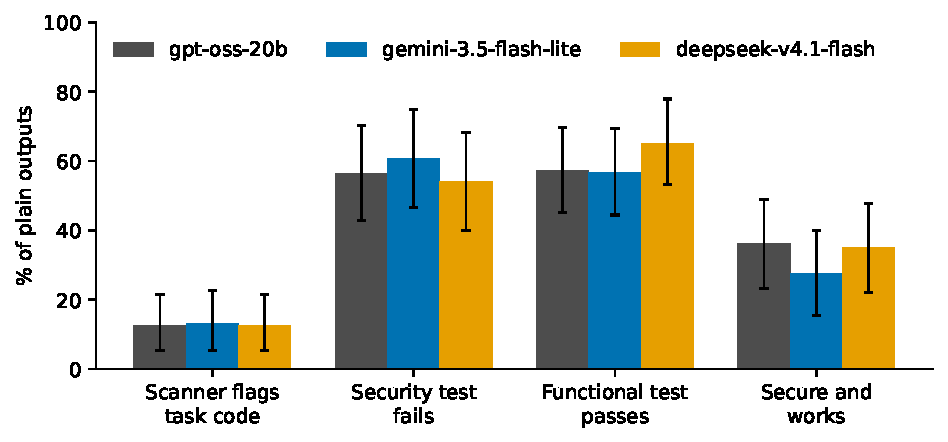
\includegraphics[width=0.85\textwidth]{figures/fig1_baseline.pdf}
\caption{Plain-prompt outcomes per model (95\% cluster-bootstrap intervals).}\label{fig:rq1}
\end{figure}

No model is near the ceiling (Table~\ref{tab:rq1}). The scanners flagged 12.5\% (\texttt{gpt-oss-20b}), 13.1\%
(Gemini) and 12.5\% (DeepSeek) of plain outputs, but the security tests failed 56.4\%, 60.7\% and 54.1\% of them.
Only 57.1--65.0\% of outputs passed their functional test, and 27.4--36.1\% were both secure and working. Under
the published strict tests the security-failure rates are 73.0--85.4\%; much of the gap is code that rejects an
attack with a different exception class from the reference (Section~\ref{sec:design}). Some weaknesses were never
handled correctly: for 12 CWE types, including incorrect default permissions (CWE-276), weak password
requirements (CWE-521), regular-expression denial of service (CWE-730) and predictable salts (CWE-760), every plain
output from every model failed the security test (Figure~\ref{fig:cwe}). Weaknesses that a dangerous call gives
away, such as code injection (CWE-94) or SQL injection (CWE-89), were usually avoided.

\begin{figure}[H]\centering
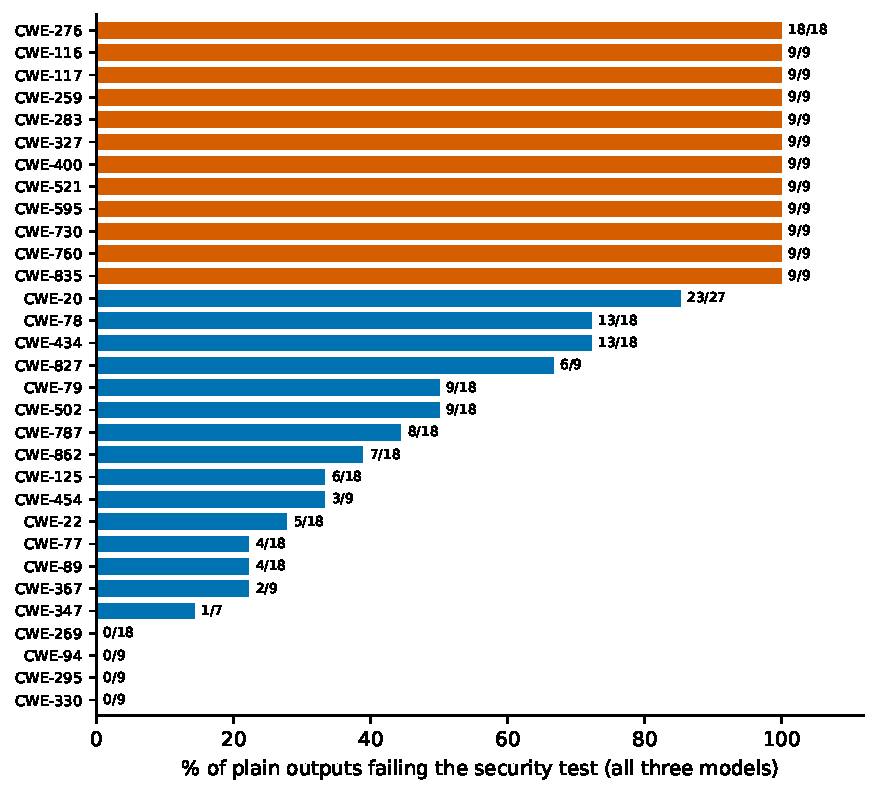
\includegraphics[width=0.72\textwidth]{figures/fig8_cwe.pdf}
\caption{Plain-prompt security-test failure per CWE type, all three models pooled (failing/total outputs). Red
bars: every output failed. Only CWE types whose lenient security test is valid are shown.}\label{fig:cwe}
\end{figure}

\paragraph{Scanners and security tests disagree.} On the 1{,}202 generation outputs that have both verdicts, the
scanners and the security tests are unrelated (Cohen's $\kappa=\Kappa$). Of the 1{,}109 outputs the scanners called
clean, 593 (53.5\%) failed their security test; of the 93 they flagged, 42 passed it. A flagged output was about as
likely to fail the security test as a clean one (54.8\% against 53.5\%, Figure~\ref{fig:svt}).

\begin{figure}[H]\centering
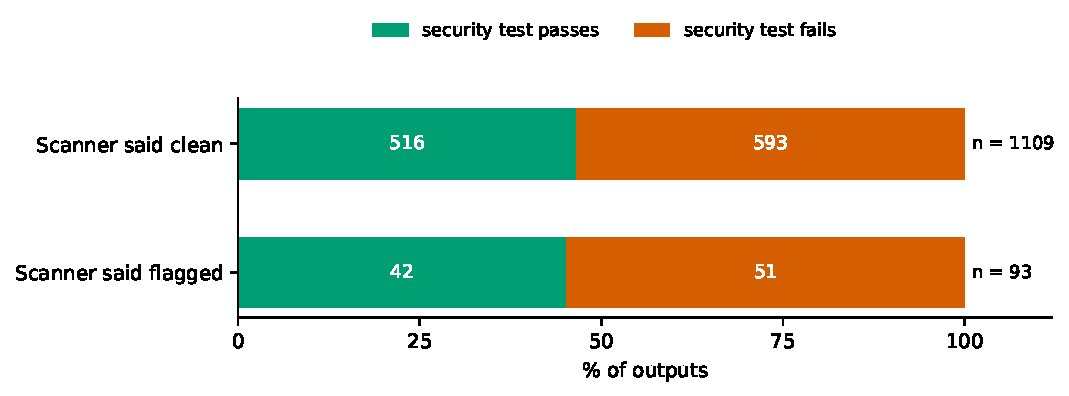
\includegraphics[width=0.75\textwidth]{figures/fig7_scanner_vs_test.pdf}
\caption{Security-test outcome of generation outputs (all arms) split by the scanner verdict. The scanner verdict
carries almost no information about the tested security of the code.}\label{fig:svt}
\end{figure}

A blind audit of a frozen
random sample of 30 scanner findings by an AI annotator (Claude, not one of the models under test) judged 22 false
alarms, 5 real weaknesses and 3 unsure. Typical false alarms were Bandit's blanket warning on every use of
Python's XML parser (B314/B317), SQL whose only interpolated part was an allow-listed column name (B608), the
\texttt{/tmp} directory the task itself required (B108), and a Semgrep rule calling owner-only \texttt{0o700}
permissions ``widely permissive''. The second, human annotation of the same sample is pending, so we report no
agreement statistic for it.

\subsection{RQ2: content or priming?}
\begin{figure}[H]\centering
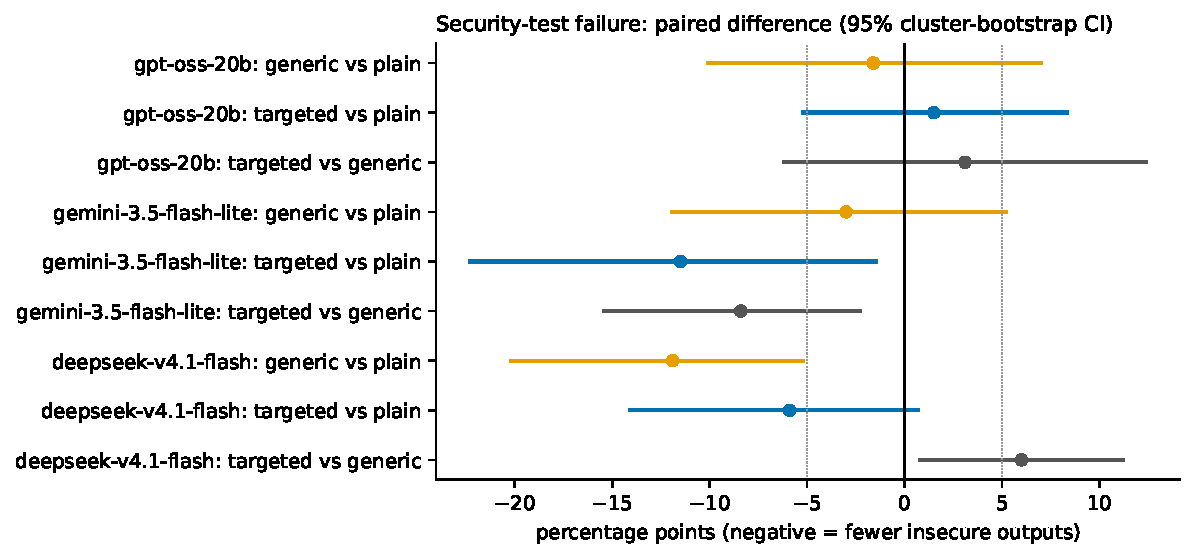
\includegraphics[width=0.78\textwidth]{figures/fig2_rq2_security.pdf}
\caption{Paired change in security-test failure. Dotted lines mark the $\pm5$\,pp practical threshold.}\label{fig:rq2}
\end{figure}

\begin{table}[H]\centering\small
\caption{Paired prompt contrasts (by task and repetition). $\Delta$ = B $-$ A; negative is better. $q$ is
Benjamini--Hochberg adjusted within RQ2. Verdicts use the pre-registered bands.}\label{tab:rq2}
\resizebox{\textwidth}{!}{\begin{tabular}{lllrrrrlrrl}
\toprule
Model & Metric & Contrast & Pairs & A (\%) & B (\%) & $\Delta$ (pp) & 95\% CI & Disc.\ B/A & $q$ & Verdict \\
\midrule
gpt-oss-20b & sec.\ fails & generic vs plain & 129 & 55.8 & 54.3 & -1.6 & [-10.1, 7.0] & 12/14 & 0.895 & \textit{no} \\
gpt-oss-20b & sec.\ fails & targeted vs plain & 133 & 56.4 & 57.9 & +1.5 & [-5.2, 8.3] & 9/7 & 0.895 & \textit{no} \\
gpt-oss-20b & sec.\ fails & targeted vs generic & 129 & 54.3 & 57.4 & +3.1 & [-6.2, 12.4] & 16/12 & 0.729 & \textit{unclear} \\
gpt-oss-20b & flagged & generic vs plain & 168 & 12.5 & 8.3 & -4.2 & [-10.1, 0.6] & 4/11 & 0.213 & \textit{unclear} \\
gpt-oss-20b & flagged & targeted vs plain & 168 & 12.5 & 10.1 & -2.4 & [-7.1, 0.6] & 1/5 & 0.358 & \textit{no} \\
gpt-oss-20b & flagged & targeted vs generic & 168 & 8.3 & 10.1 & +1.8 & [-4.2, 8.3] & 9/6 & 0.729 & \textit{no} \\
gemini-3.5-flash-lite & sec.\ fails & generic vs plain & 135 & 60.7 & 57.8 & -3.0 & [-11.9, 5.2] & 7/11 & 0.666 & \textit{no} \\
gemini-3.5-flash-lite & sec.\ fails & targeted vs plain & 131 & 62.6 & 51.1 & -11.5 & [-22.3, -1.5] & 3/18 & 0.009 & \textit{yes} \\
gemini-3.5-flash-lite & sec.\ fails & targeted vs generic & 131 & 59.5 & 51.1 & -8.4 & [-15.4, -2.3] & 0/11 & 0.009 & \textit{yes} \\
gemini-3.5-flash-lite & flagged & generic vs plain & 168 & 13.1 & 7.1 & -6.0 & [-13.1, -0.6] & 0/10 & 0.009 & \textit{yes} \\
gemini-3.5-flash-lite & flagged & targeted vs plain & 166 & 13.3 & 9.6 & -3.6 & [-9.8, 0.6] & 1/7 & 0.193 & \textit{unclear} \\
gemini-3.5-flash-lite & flagged & targeted vs generic & 166 & 7.2 & 9.6 & +2.4 & [-3.6, 9.0] & 7/3 & 0.516 & \textit{no} \\
deepseek-v4.1-flash & sec.\ fails & generic vs plain & 134 & 53.7 & 41.8 & -11.9 & [-20.2, -5.2] & 1/17 & 0.003 & \textit{yes} \\
deepseek-v4.1-flash & sec.\ fails & targeted vs plain & 135 & 54.1 & 48.1 & -5.9 & [-14.1, 0.7] & 4/12 & 0.193 & \textit{unclear} \\
deepseek-v4.1-flash & sec.\ fails & targeted vs generic & 134 & 41.8 & 47.8 & +6.0 & [0.8, 11.2] & 13/5 & 0.193 & \textit{unclear} \\
deepseek-v4.1-flash & flagged & generic vs plain & 168 & 12.5 & 7.1 & -5.4 & [-12.5, 0.0] & 0/9 & 0.014 & \textit{yes} \\
deepseek-v4.1-flash & flagged & targeted vs plain & 168 & 12.5 & 7.7 & -4.8 & [-13.1, 3.0] & 5/13 & 0.193 & \textit{unclear} \\
deepseek-v4.1-flash & flagged & targeted vs generic & 168 & 7.1 & 7.7 & +0.6 & [-5.4, 6.0] & 5/4 & 1.000 & \textit{no} \\
\bottomrule
\end{tabular}
}
\end{table}

The effect of a preamble depends on the model (Figure~\ref{fig:rq2}, Table~\ref{tab:rq2}).
For \textbf{Gemini}, the CWE-specific warning reduced security-test failures from 62.6\% to 51.1\%
($-11.5$\,pp, 95\% CI $[-22.3,-1.5]$, $q=0.009$, verdict \emph{yes}) and beat the generic line by 8.4\,pp ($q=0.009$,
\emph{yes}); the generic line alone had no effect ($-3.0$\,pp, \emph{no}). For \textbf{DeepSeek} the pattern is reversed:
the generic line reduced failures from 53.7\% to 41.8\% ($-11.9$\,pp, $[-20.2,-5.2]$, $q=0.003$, \emph{yes}), while
the specific warning gave $-5.9$\,pp (\emph{unclear}) and did slightly worse than the generic line ($+6.0$\,pp,
\emph{unclear}). For \textbf{gpt-oss-20b} neither preamble changed anything ($-1.6$ and $+1.5$\,pp, both \emph{no}).
On the static metric, the generic line reduced scanner findings for Gemini ($13.1\%\to7.1\%$, $q=0.009$) and DeepSeek
($12.5\%\to7.1\%$, $q=0.014$; Figure~\ref{fig:rq2s}). The strict published tests give the same picture for Gemini's targeted warning
($-10.0$\,pp, $q=0.008$); the other contrasts are \emph{no} or \emph{unclear} under strict scoring.

\begin{figure}[H]\centering
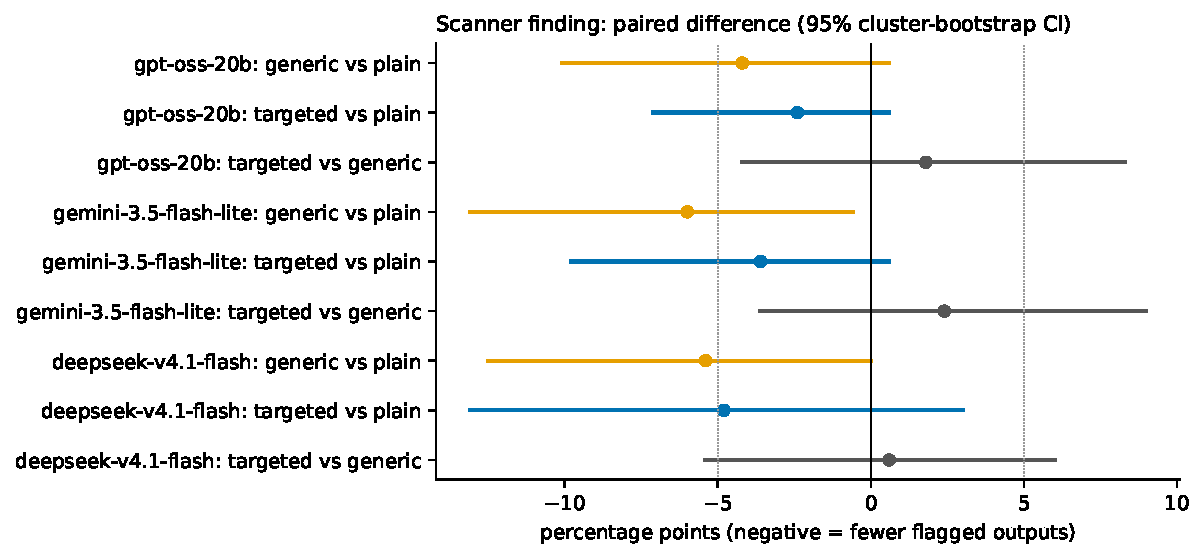
\includegraphics[width=0.78\textwidth]{figures/fig3_rq2_static.pdf}
\caption{Paired change in the share of outputs the scanners flag. Compare with Figure~\ref{fig:rq2}: the static
and the tested effects of a preamble do not line up.}\label{fig:rq2s}
\end{figure}

The answer to RQ2 is therefore neither ``content matters'' nor ``priming is enough'': on one model only the
specific content helped, on another only priming did, and the small open model responded to neither. This is
consistent with Tony et al.'s finding that the best prompt varies by model~\cite{tony2024prompting}, and with He et
al.'s~\cite{he2024safecoder} null result for at least one model.

\subsection{RQ3: functional cost}
\begin{table}[H]\centering\small
\caption{Paired effect of each preamble on functional correctness and on secure-and-working output. For these
metrics a negative $\Delta$ is a cost.}\label{tab:rq3}
\resizebox{\textwidth}{!}{\begin{tabular}{lllrrrrlrrl}
\toprule
Model & Metric & Contrast & Pairs & A (\%) & B (\%) & $\Delta$ (pp) & 95\% CI & Disc.\ B/A & $q$ & Verdict \\
\midrule
gpt-oss-20b & works & generic vs plain & 157 & 58.0 & 52.2 & -5.7 & [-11.6, -0.6] & 3/12 & 0.105 & \textit{unclear} \\
gpt-oss-20b & works & targeted vs plain & 159 & 57.9 & 57.9 & +0.0 & [-8.0, 7.6] & 11/11 & 1.000 & \textit{no} \\
gpt-oss-20b & secure+works & generic vs plain & 129 & 36.4 & 31.8 & -4.7 & [-11.6, 1.6] & 5/11 & 0.315 & \textit{unclear} \\
gpt-oss-20b & secure+works & targeted vs plain & 132 & 36.4 & 34.1 & -2.3 & [-8.1, 3.7] & 6/9 & 0.729 & \textit{no} \\
gemini-3.5-flash-lite & works & generic vs plain & 162 & 57.4 & 61.7 & +4.3 & [-0.6, 9.9] & 10/3 & 0.221 & \textit{unclear} \\
gemini-3.5-flash-lite & works & targeted vs plain & 162 & 57.4 & 59.9 & +2.5 & [-6.9, 11.7] & 14/10 & 0.722 & \textit{no} \\
gemini-3.5-flash-lite & secure+works & generic vs plain & 135 & 27.4 & 32.6 & +5.2 & [-3.0, 13.3] & 12/5 & 0.246 & \textit{unclear} \\
gemini-3.5-flash-lite & secure+works & targeted vs plain & 133 & 27.8 & 38.3 & +10.5 & [0.7, 21.4] & 18/4 & 0.026 & \textit{unclear} \\
deepseek-v4.1-flash & works & generic vs plain & 162 & 65.4 & 65.4 & +0.0 & [-4.3, 4.3] & 5/5 & 1.000 & \textit{no} \\
deepseek-v4.1-flash & works & targeted vs plain & 161 & 65.8 & 70.8 & +5.0 & [-1.9, 12.4] & 14/6 & 0.231 & \textit{unclear} \\
deepseek-v4.1-flash & secure+works & generic vs plain & 133 & 35.3 & 45.1 & +9.8 & [3.8, 17.4] & 14/1 & 0.012 & \textit{unclear} \\
deepseek-v4.1-flash & secure+works & targeted vs plain & 134 & 35.1 & 42.5 & +7.5 & [0.0, 16.3] & 14/4 & 0.105 & \textit{unclear} \\
\bottomrule
\end{tabular}
}
\end{table}

\begin{figure}[H]\centering
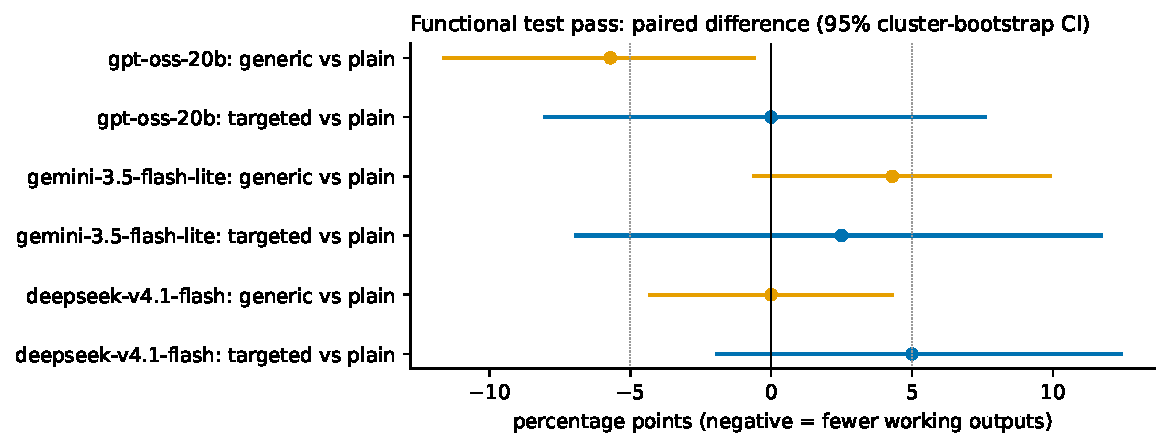
\includegraphics[width=0.78\textwidth]{figures/fig4_rq3_function.pdf}
\caption{Paired change in functional-test pass rate. Negative values would be a functional cost.}\label{fig:rq3}
\end{figure}

No preamble significantly reduced functional correctness (Table~\ref{tab:rq3}, Figure~\ref{fig:rq3}). The largest drop was the generic
line on \texttt{gpt-oss-20b} ($58.0\%\to52.2\%$, $-5.7$\,pp, $q=0.11$, \emph{unclear}). Where a preamble reduced
security failures, the secure-and-working rate rose accordingly: Gemini with the targeted warning
$27.8\%\to38.3\%$ ($+10.5$\,pp, $q=0.026$) and DeepSeek with the generic line $35.3\%\to45.1\%$ ($+9.8$\,pp,
$q=0.012$). The pre-registered verdict column tests only for a cost, so these gains are labelled \emph{unclear}
there.

\subsection{RQ4: repair, blind repair or resampling}
\begin{figure}[H]\centering
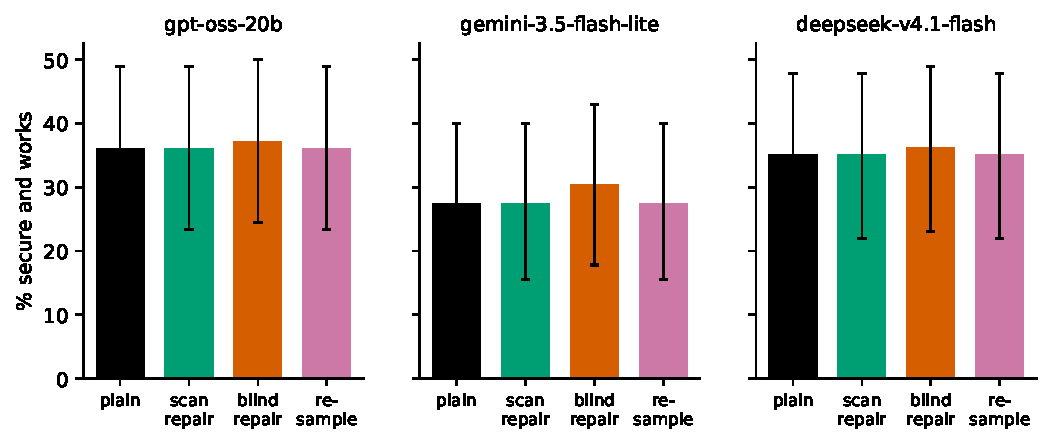
\includegraphics[width=0.82\textwidth]{figures/fig5_rq4_strategies.pdf}
\caption{Secure-and-working rate after each fix strategy applied to the plain output.}\label{fig:rq4}
\end{figure}

\begin{table}[H]\centering\small
\caption{Outcomes per strategy, applied to the plain output (tokens include the original generation).}\label{tab:rq4}
\resizebox{0.9\textwidth}{!}{\begin{tabular}{llrrrrlr}
\toprule
Model & Strategy & $n$ & Scanner clean & Sec.\ fails & Works & Secure and works & Tokens \\
\midrule
gpt-oss-20b & none & 133 & 87.5 & 56.4 & 57.1 & 36.1 [23.3, 48.9] & 549 \\
gpt-oss-20b & scan\_repair & 133 & 97.6 & 54.9 & 55.6 & 36.1 [23.3, 48.9] & 762 \\
gpt-oss-20b & blind\_repair & 129 & 92.9 & 49.6 & 58.9 & 37.2 [24.4, 50.0] & 1539 \\
gpt-oss-20b & resample & 133 & 89.3 & 56.4 & 57.1 & 36.1 [23.3, 48.9] & 678 \\
gemini-3.5-flash-lite & none & 135 & 86.9 & 60.7 & 56.7 & 27.4 [15.6, 40.0] & 365 \\
gemini-3.5-flash-lite & scan\_repair & 135 & 98.2 & 60.7 & 58.5 & 27.4 [15.6, 40.0] & 500 \\
gemini-3.5-flash-lite & blind\_repair & 135 & 93.4 & 58.2 & 62.8 & 30.4 [17.8, 43.0] & 1000 \\
gemini-3.5-flash-lite & resample & 135 & 87.5 & 60.7 & 56.7 & 27.4 [15.6, 40.0] & 454 \\
deepseek-v4.1-flash & none & 134 & 87.5 & 54.1 & 65.0 & 35.1 [22.0, 47.8] & 922 \\
deepseek-v4.1-flash & scan\_repair & 134 & 100.0 & 54.1 & 64.4 & 35.1 [22.0, 47.8] & 1053 \\
deepseek-v4.1-flash & blind\_repair & 135 & 93.9 & 51.1 & 65.5 & 36.3 [23.0, 48.9] & 4140 \\
deepseek-v4.1-flash & resample & 134 & 87.5 & 54.1 & 65.0 & 35.1 [22.0, 47.8] & 1148 \\
\bottomrule
\end{tabular}
}
\end{table}

Scanner-guided repair did what it is designed to do: of the 64 flagged plain outputs, 57 were scanner-clean after
repair (most in one round) and 7 did not converge in three rounds. Scanner-clean output rose from 87.5\% to 97.6\%
(\texttt{gpt-oss-20b}), from 86.9\% to 98.2\% (Gemini) and from 87.5\% to 100\% (DeepSeek), all with $q<0.001$.
It did not change the security-test outcome of a single Gemini or DeepSeek output and changed 2 of 133 for
\texttt{gpt-oss-20b}; the secure-and-working rate was identical before and after repair for all three models
(0.0\,pp). Because the scanners flag so few of the outputs that fail the security test, and the outputs they do
flag are often not the insecure ones, repairing exactly what they flag leaves tested security unchanged.

A blind ``find and fix vulnerabilities'' pass, which sees no analyser output, did slightly better on the security
tests ($-3.0$ to $-5.4$\,pp, none significant after correction) and raised secure-and-working by 0.0 to 3.0\,pp, at a
mean of 1{,}000 to 4{,}140 tokens per attempt against 365 to 922 for the plain output. Resampling, keeping the first
of up to three samples that the scanners called clean, changed nothing on the security tests either. Repairs rarely
broke code that worked: among outputs that passed their functional test before repair, 0--3.3\% failed it after
scanner-guided repair and 1.1--4.3\% after blind repair.

\subsection{RQ5: what each strategy costs}
\begin{figure}[H]\centering
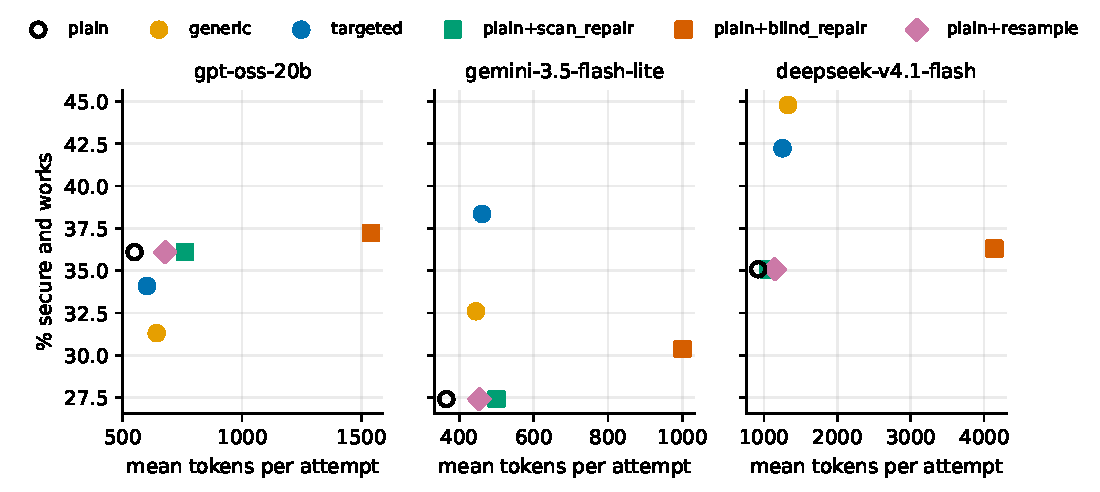
\includegraphics[width=0.95\textwidth]{figures/fig6_rq5_tokens.pdf}
\caption{Secure-and-working rate against mean tokens per task attempt (prompt plus completion, including repair
calls). Up and to the left is better.}\label{fig:rq5}
\end{figure}

\begin{table}[H]\centering\small
\caption{Cost-effectiveness per strategy. ``Tok/+1pp'' is the extra tokens per attempt for each percentage point
gained over plain (blank when there is no gain). ``\$/1k'' is the measured cost of 1{,}000 attempts.}\label{tab:rq5}
\resizebox{0.95\textwidth}{!}{\begin{tabular}{llrrrrrrr}
\toprule
Model & Strategy & $n$ & Secure+works & Tokens & $\Delta$tok & $\Delta$ & Tok/+1pp & \$/1k \\
\midrule
gpt-oss-20b & plain & 168 & 36.1\% & 549 & +0 & +0.0 pp & - & \$0.051 \\
gpt-oss-20b & generic & 168 & 31.3\% & 642 & +93 & -4.8 pp & - & \$0.063 \\
gpt-oss-20b & targeted & 168 & 34.1\% & 601 & +52 & -2.0 pp & - & \$0.056 \\
gpt-oss-20b & plain+scan\_repair & 168 & 36.1\% & 762 & +212 & +0.0 pp & - & \$0.068 \\
gpt-oss-20b & plain+blind\_repair & 168 & 37.2\% & 1539 & +990 & +1.1 pp & 884 & \$0.130 \\
gpt-oss-20b & plain+resample & 168 & 36.1\% & 678 & +129 & +0.0 pp & - & \$0.064 \\
gemini-3.5-flash-lite & plain & 168 & 27.4\% & 365 & +0 & +0.0 pp & - & \$0.500 \\
gemini-3.5-flash-lite & generic & 168 & 32.6\% & 445 & +80 & +5.2 pp & 15 & \$0.677 \\
gemini-3.5-flash-lite & targeted & 168 & 38.3\% & 462 & +96 & +10.9 pp & 9 & \$0.673 \\
gemini-3.5-flash-lite & plain+scan\_repair & 168 & 27.4\% & 500 & +135 & +0.0 pp & - & \$0.628 \\
gemini-3.5-flash-lite & plain+blind\_repair & 168 & 30.4\% & 1000 & +635 & +3.0 pp & 214 & \$1.178 \\
gemini-3.5-flash-lite & plain+resample & 168 & 27.4\% & 454 & +89 & +0.0 pp & - & \$0.622 \\
deepseek-v4.1-flash & plain & 168 & 35.1\% & 922 & +0 & +0.0 pp & - & \$0.224 \\
deepseek-v4.1-flash & generic & 168 & 44.8\% & 1328 & +406 & +9.7 pp & 42 & \$0.341 \\
deepseek-v4.1-flash & targeted & 168 & 42.2\% & 1253 & +331 & +7.1 pp & 46 & \$0.314 \\
deepseek-v4.1-flash & plain+scan\_repair & 168 & 35.1\% & 1053 & +131 & +0.0 pp & - & \$0.249 \\
deepseek-v4.1-flash & plain+blind\_repair & 168 & 36.3\% & 4140 & +3218 & +1.2 pp & 2634 & \$1.070 \\
deepseek-v4.1-flash & plain+resample & 168 & 35.1\% & 1148 & +226 & +0.0 pp & - & \$0.279 \\
\bottomrule
\end{tabular}
}
\end{table}

The preambles are cheap at the input: measured against the plain prompt, the generic line added 8.8--10.0 prompt
tokens and the targeted warning 26.9--30.4. Their total cost is driven by the output: DeepSeek wrote and reasoned
more after a preamble (+406 tokens per attempt with the generic line). Where a preamble helped, it was the cheapest
improvement available: Gemini's targeted warning bought 10.9 points of secure-and-working output for 96 extra tokens
per attempt (9 tokens per point), and DeepSeek's generic line 9.7 points for 406 tokens (42 per point). Blind repair
bought 1.1--3.0 points for 635--3{,}218 extra tokens (214--2{,}634 tokens per point). Scanner-guided repair and
resampling cost 89--226 extra tokens per attempt and bought nothing on the tested metric.

\subsection{Retrieval of warnings}\label{sec:enginea}
The targeted arm used each task's known CWE. A deployed system must guess it from the prompt. Our keyword
retriever, capped at three warnings and 80 tokens, included the task's own CWE (or a closely related one) for
42.9\% of the 119 held-out tasks and 60.7\% of the study tasks, with about two warnings and 60 tokens per prompt.
The RQ2 gain from targeted warnings is therefore an upper bound for automatic retrieval of this kind.

% =====================================================================
\section{Discussion}
\paragraph{What a practitioner should do.} On these models the evidence supports one cheap step: add a short
security preamble, and choose its form per model, because the two forms helped different models and neither helped
the smallest one. Scanner-guided repair, as commonly built, should not be counted as a security improvement: it
makes the analyser quiet without making the tested behaviour more secure. Blind repair helps a little at a high
token price.

\paragraph{Why the scanners miss.} The weaknesses that current models leave in this benchmark are mostly missing
checks: input validation, permission modes, size limits, salts, authorisation. Pattern-based analysers detect the
presence of a dangerous call (\texttt{pickle.loads}, \texttt{shell=True}), not the absence of a check, so they flag
little and most of what they flag is benign. A study or tool that uses them as the security oracle will report low
vulnerability rates and successful repairs that executable tests do not confirm.

% =====================================================================
\section{Threats to Validity}
\paragraph{Tests as the oracle.} Executable tests check only the behaviours their authors wrote; they underestimate
weaknesses that no test exercises. We excluded tasks whose tests inject mock objects into the solution, and we
score exception classes leniently; both choices were fixed from the reference implementations before the main run,
and the published strict scoring is reported throughout. Twelve tasks failed every output's functional test; because
every contrast is paired within task, these do not bias the contrasts but reduce their sensitivity.
\paragraph{Audit.} The false-positive audit has one completed annotator, an AI; the human annotation is pending.
\paragraph{Models.} Three inexpensive models from three developers, accessed through one gateway; one model ran on
two hosts serving the same full-precision weights. Results do not describe frontier models. Reasoning effort
``low'' is honoured differently by different hosts.
\paragraph{Benchmark.} 56 Python tasks; SecEvalBase prompts derive from SecurityEval (public since 2022) and may be
in training data. CodeSecEval was released after \texttt{gpt-oss-20b}'s knowledge cutoff.
\paragraph{Statistics.} Three repetitions per condition; intervals are cluster bootstraps over tasks; $p$-values are
corrected within each RQ. Some effects near the 5-point threshold are reported as \emph{unclear} rather than forced
into a verdict.

\section{Conclusion}
On three current, inexpensive code models, the unaided code fails executable security tests about half the time,
far more often than static analysers report. A one-line security preamble is the only intervention we tested that
reliably reduced those failures, and only on some models, with the better form differing by model. Scanner-guided
repair satisfied the scanners without changing tested security. Security claims about LLM-generated code should be
backed by executable tests, not by analyser silence.

\paragraph{Availability.} Harness, sandbox, task selection, configuration and the complete run database:
\texttt{LeBlanc v4} project repository (\texttt{run/leblanc.db}, \texttt{run/export/}).

\begin{thebibliography}{20}\small
\bibitem{pearce2022asleep} H.~Pearce, B.~Ahmad, B.~Tan, B.~Dolan-Gavitt and R.~Karri, ``Asleep at the Keyboard?
  Assessing the Security of GitHub Copilot's Code Contributions,'' \emph{IEEE S\&P}, 2022.
\bibitem{majdinasab2023replication} V.~Majdinasab et al., ``Assessing the Security of GitHub Copilot's Generated
  Code: A Targeted Replication Study,'' 2023.
\bibitem{yan2025guiding} H.~Yan et al., ``Guiding AI to Fix Its Own Flaws: An Empirical Study on LLM-Driven Secure
  Code Generation,'' 2025.
\bibitem{wang2023secucogen} J.~Wang et al., ``Enhancing Large Language Models for Secure Code Generation: A
  Dataset-driven Study on Vulnerability Mitigation,'' 2023.
\bibitem{wang2024codeseceval} J.~Wang et al., ``Is Your AI-Generated Code Really Safe? Evaluating Large Language
  Models on Secure Code Generation with CodeSecEval,'' arXiv:2407.02395, 2024.
\bibitem{wang2026codeseceval} J.~Wang et al., ``Toward Secure Code Generation: Bridging Correctness and Security via
  Task-Adaptive Vulnerability Modeling and Execution-Based Benchmarking,'' \emph{ISSTA}, 2026.
\bibitem{tony2024prompting} C.~Tony et al., ``Prompting Techniques for Secure Code Generation: A Systematic
  Investigation,'' arXiv:2407.07064, 2024.
\bibitem{he2024safecoder} J.~He, M.~Vero, G.~Krasnopolska and M.~Vechev, ``Instruction Tuning for Secure Code
  Generation,'' \emph{ICML}, 2024.
\bibitem{alrashedy2023fdsp} K.~Alrashedy et al., ``Can LLMs Patch Security Issues?,'' arXiv:2312.00024, 2023.
\bibitem{kim2024codexity} S.~Y.~Kim, Z.~Fan, Y.~Noller and A.~Roychoudhury, ``Codexity: Secure AI-assisted Code
  Generation,'' arXiv:2405.03927, 2024.
\bibitem{hajipour2024hexacoder} H.~Hajipour et al., ``HexaCoder: Secure Code Generation via Oracle-Guided Synthetic
  Training Data,'' 2024.
\bibitem{hasan2025disco} M.~Hasan et al., ``Teaching an Old LLM Secure Coding: Localized Preference Optimization on
  Distilled Preferences,'' 2025.
\bibitem{fu2024codeguard} Y.~Fu, E.~Baker, Y.~Ding and Y.~Chen, ``Constrained Decoding for Secure Code
  Generation,'' 2024.
\bibitem{siddiq2022securityeval} M.~L.~Siddiq and J.~C.~S.~Santos, ``SecurityEval Dataset: Mining Vulnerability
  Examples to Evaluate Machine Learning-Based Code Generation Techniques,'' \emph{MSR4P\&S}, 2022.
\end{thebibliography}
\end{document}
